\subsection{WebSocket 通信流程实现}

FoodShield 使用 Flask-SocketIO 实现用户端与骑手端之间的订单级实时通信。系统以订单号作为通信房间标识，每个订单对应一个独立的 WebSocket Room。用户和骑手只有通过各自的入房认证后，才能加入对应订单房间并发送或接收消息。

用户端入房时触发 \texttt{join\_order} 事件，并提交 \texttt{order\_id}、\texttt{token} 和角色信息。服务器校验 Token 成功后执行 \texttt{join\_room(order\_id)}，将当前连接加入订单房间。骑手端入房时触发 \texttt{join\_order\_as\_rider} 事件，服务器检查订单是否存在以及订单状态是否允许通信，校验通过后将骑手连接加入同一订单房间。

消息发送时，前端触发 \texttt{send\_message} 事件，将订单号、发送方角色和消息内容发送到服务器。服务器接收到消息后，依次完成以下操作：

\begin{enumerate}
    \item 检查订单号是否有效；
    \item 生成全局唯一消息编号 \texttt{msg\_id}；
    \item 生成 ISO 8601 格式时间戳；
    \item 对消息明文执行 SM4-CBC 加密；
    \item 对订单号、发送方标识、角色、明文内容和时间戳计算 SM3 消息摘要；
    \item 将密文、消息摘要和元数据写入 \texttt{messages} 表；
    \item 更新该订单对应的 Merkle Root 快照；
    \item 将消息广播给同一订单房间内的用户端和骑手端。
\end{enumerate}

通信流程可以抽象为以下流程图：

\begin{figure}[H]
    \centering
    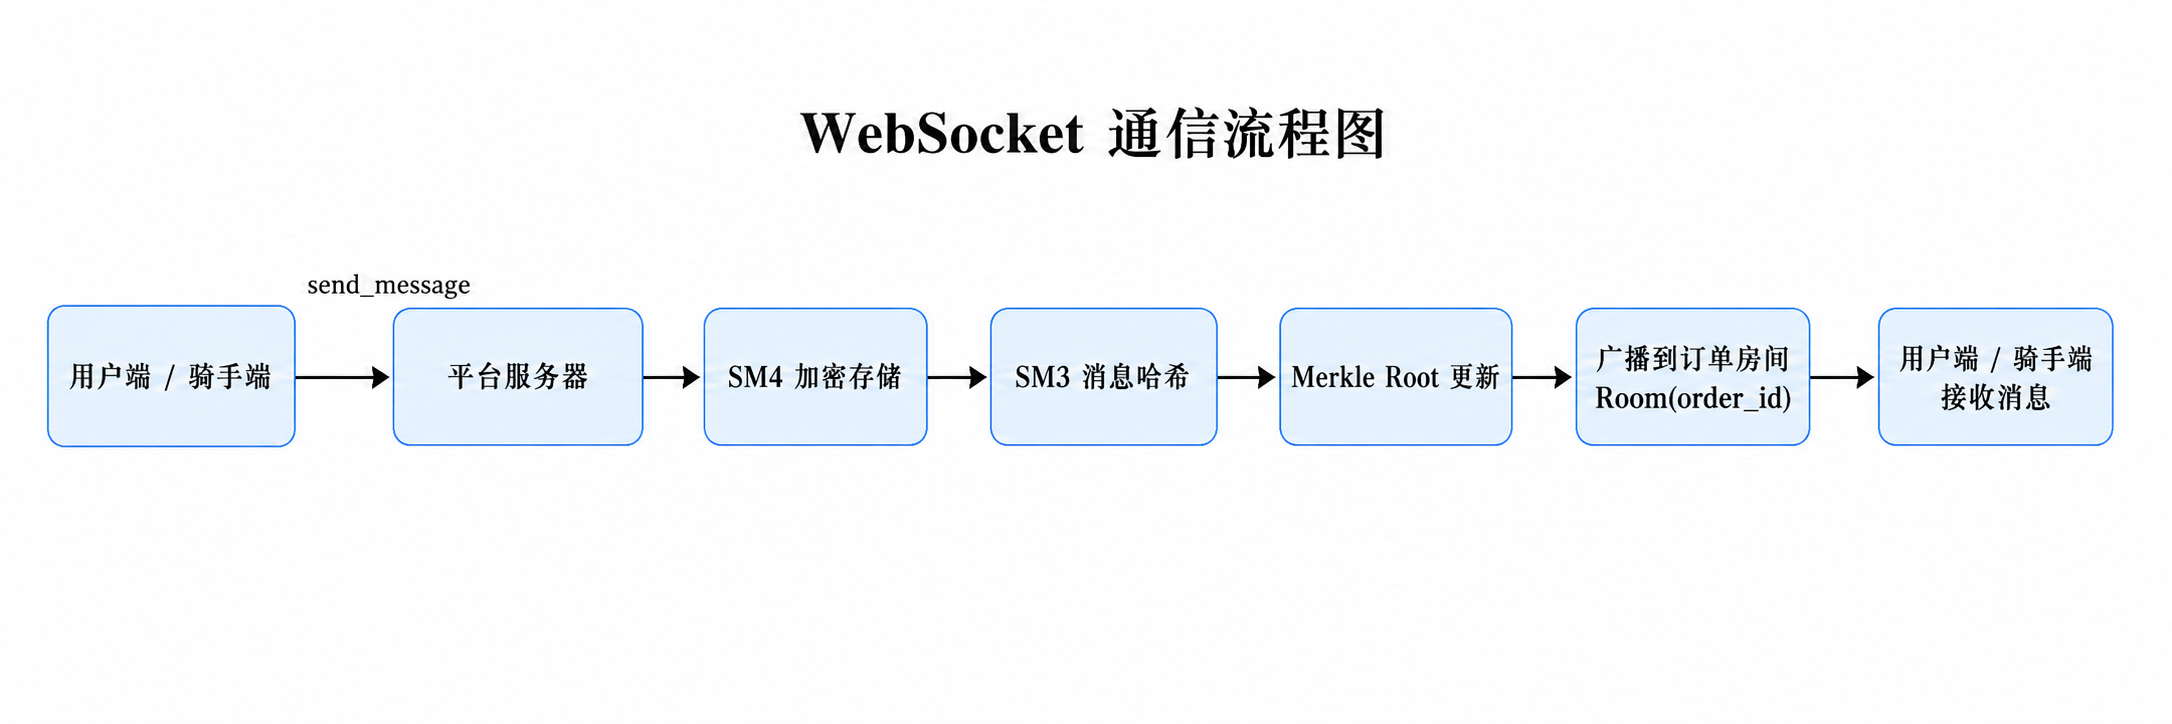
\includegraphics[width=0.85\textwidth]{content/chapter4/websocket_flow.png}
    \caption{订单级 WebSocket 通信流程}
    \label{fig:websocket-flow}
\end{figure}

通过订单房间隔离机制，不同订单之间的消息不会相互传播。通过后端统一转发机制，系统能够在消息进入数据库前同步完成加密、哈希和审计操作，使普通聊天流程和安全机制形成联动，而不是在聊天结束后再额外补做安全处理。
